\documentclass[../linear-spaces.tex]{subfiles}

\begin{document}

\chapter{Introduction}
\section{Definition of a linear space}
Let $V$ be a non-empty set of objects, called \textit{elements}. The set V is
called linear space if it satisfies the following ten axioms, which are stated
in three groups.

\section*{Axioms of a linear space}

\begin{list}{Axiom}{}
    \item 1.\textit{ Closure property of addition}: for every pair of elements $x,y\in V$, their sum is written as $z=x+y$ and $z\in V$.
    \item 2.\textit{ Closure property of scalar product}: for any $x\in V$ and $a\in\mathbb R$, there is an element $z=ax\in V$.
\end{list}

\subsection*{Axioms for addition}

There are four axioms of addition, we will use a number and a letter to refer
to them. However if we are talking of addition properties we will simply use a
letter to reference them. The same will be done for the axioms of scalar
products.

\begin{list}{Axiom}{}
    \item 3.a.\textit{ Commutative law}: for any $x,y\in V$, we have $x+y = y+x$.
    \item 4.b.\textit{ Associative law}: for any $x,y,z\in V$, we have $(x+y) + z = x + (y + z)$.
    \item 5.c.\textit{ Existence of zero as an element}: there is a number in $V$, designated as $O$ (big `o'), that satisfies
    \[
        x + O = x,\quad \forall x \in V
        \]
        
        \item 6.d.\textit{ Opposite elements}: for all $x\in V$, the element $(-1)x$ has the property
        \[
            x + (-1)x = O
            \]
        \end{list}
        
        \subsection*{Axioms for scalar product}
        \begin{list}{Axiom}{}
            
            \item 7.a.\textit{ Associative law}: for all $x \in V$ and every pair $a,b\in \mathbb R$, we have
            
            \[
                a(bx) = (ab)x
                \]
                
                \item 8.b.\textit{ Distributive law for addition in $V$}: for all $x,y\in V$ and $a\in \mathbb{R}$, it is true that
                
                \[
                    a(x+y) = ax+ay
                    \]
                    
                    \item 9.c.\textit{ Distributive law for addition in $\mathbb R$}: for any $x\in V$ and $a,b\in\mathbb{R}$, we have
                    
                    \[
                        (a+b)x = ax+bx
                        \]
                        
                        \item 10.d.\textit{ Existence of an identical element}: for all $x\in V$ theres an unique element $I$ such that $Ix=x$
                        (commonly this element is $1$. But, for example, the identical element in matrix spaces is called \textit{identity matrix},
                        defined as $I=\textnormal{diag}(1)$)
                    \end{list}
                    
                    \section{Examples of linear spaces}
                    
                    The following examples can be proven to be linear spaces
                    
                    \begin{enumerate}
                        \item Real numbers
                        \item The vector space of real numbers $\mathbb R^n$
                        \item The set of all matrices
                        \item Polynomials $P$ with $\deg P \leq n$ (in this case, if $\deg P = n$, we would
                        have a problem with axioms of additions. We can't ensure the sum of two
                        polynomials of degree $n$ has degree $n$).
                        \item The set of all polynomials
                        \item The set of continuous functions on an interval $\left[a, b\right]$. This space
                        is designated as $C(a,b)$.
                        \item The set of all integrable functions on an interval
                        \item The set of differentiable functions on an interval
                        \item A plane in $\mathbb R^3$ with the equation $ax+by+cz=0$. Note that this plane
                        must always go through the origin to be a linear space.
                    \end{enumerate}
                    
                    There are plenty of examples for linear spaces. We can ``create'' a linear
                    space if we define addition and multiplication for that space.

\section{Consequences of the axioms}

The following theorems are a consequence of the axioms of linear space.

\begin{theorem}[Uniqueness of `O']
    In any linear space there is one and only one zero element
\end{theorem}

\begin{proof}
    Axiom 5 ensures that there is at least one `O' in $V$. Now,
    suppose there are two zeroes in $V$. Let $x = O_1$ and $O_2 = O$,
    thus $x + O = x + O_2 = x = O_1$, but as $O_1$ is zero, $O_1 + O_2 = O_2$,
    this means that $O_1=O_2=O$
\end{proof}

\begin{theorem}[Uniqueness of opposites]
    In any linear space each $x$ has one and only one opposite $y$ such that $x+y=O$
\end{theorem}

\begin{proof}
    Axiom 6 ensures there is at least one opposite of $x$ in $V$. Let $y_1,y_2\in V$
    be two different opposite elements for $x$. Then $x+y_1=O$ and $x+y_2=O$, then

    \[
        (x + y_1) + y_2 = y_2 + O = y_2
    \]

    and

    \[
        y_1 + (x+y_2) = y_1 + O = y_1
    \]

    Thus $y_1 + (x+y_2) = y_1 + (x+y_1) = y_1 + O = O + y_1$, this proves that $y_1
        = y_2$.
\end{proof}

\section{Subspaces of a linear space}

Let $V$ be a linear space and let $S$ be a subset of $V$, if $S$ is also a
linear space, then we say that ``$S$ is a subspace of $V$''.

A subset of a linear space if a subspace only if it satisfies the axioms of
closure.

\begin{theorem}
    Let $V$ be a linear space, if $S\subset V$ and $S \neq \emptyset$ satisfies
    the ten axioms of closure then $S$ is a subspace of $V$.
\end{theorem}

The proof for this theorem is easy, and so I discarded it.

\begin{definition}
    Let $S\subset V$, and $S\neq \emptyset$, where $V$ is a linear space. If $x\in V$ and

    \[
        x=\sum_{i=1}^{k}{c_i x_i}
    \]

    where $x_1,x_2,\dots,x_k \in S$ and $c_1,c_2,\dots,c_k\in \mathbb{R}$, is
    called a \textit{linear combination of elements in $S$}. The set of linear
    combinations of the elements of $S$ satisfies the axioms of closure, so it is
    also a subspace of $V$.\textit{ We say that this subspace is generated by $S$
        and we call it the linear span of $S$, designated by $L(S)$.} If $S=\emptyset$,
    we define $L(S)=\left\{O\right\}$.
\end{definition}

\section{Dependent and independent subsets of a linear space}

In this section we introduce the concept of independence, that is important
when working with systems of linear equations, matrices, and other subjects in
linear algebra.

\begin{definition}
    Let $S$ be a set of elements of a linear space $V$. $S$ is dependent if there
    exists a finite set of distinct elements in $x_1,x_2,\dots,x_k\in S$, and a
    set of scalars $c_1,c_2,\dots,c_k$ where not all of them are zero, that satisfies
    \[
        \sum_{i=1}^{k}{c_i x_i} = 0
    \]

    A set is independent if it is not dependent. So the following

    \[
        \sum_{i=1}^{k}{c_i x_i} = 0, \quad \textit{implies } c_1 = c_2 = \cdots = c_k =0
    \]
\end{definition}

Independency and dependency are properties of sets of elements. However, we can
apply the same concepts to the elements itself. For example, a set of vectors
$v_1, v_2, \dots, v_n \in \mathbb R^{n}$ is called independent if there is
\textbf{not} a linear combination of these vectors that produce the zero
vector.

\begin{example}
    Let $u_k(t)=t^{k}$ for $k=1,2,\dots, n$ and $t\in \mathbb{R}$. The set $V=\{u_1,u_2,\dots, u_n\}$ is independent except in the subset $S$ where $t=-1$ and $n$ is odd.

    \begin{proof}
        For $S$ to be independent, there must be $c_1,c_2,\dots, c_n$, where $c_1 = c_2 = \cdots = c_n =0$ and
        \[
            \sum_{k=0}^{n}{c_k t^{k}} = 0
        \]

        To solve this, we set $c_0=c_1=\cdots=c_n$. If we define

        \[
            f(t)=\sum_{k=0}^{n}{c_k t^{k}},
        \]

        note that $f(-1)=\begin{cases}1\quad \textnormal{if $n$ is even}\\0 \quad \textnormal{if $n$ is odd}\end{cases}$
        We can draw a picture for this problem. Imagine a circle, in which we have two points. We can travel the circumference
        counterclockwise starting from $1$. We start from $1$ because in the case $n=0$, $f(-1)=1$.

        \begin{center}
            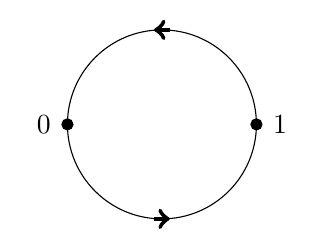
\begin{tikzpicture}
                \draw (0,0) circle(1.2cm);
                \draw[fill=black] (1.2,0) circle[radius=2pt];
                \draw[fill=black] (-1.2,0) circle[radius=2pt];
                \draw[->, ultra thick] (0.1,1.2)--(-0.1,1.2);
                \draw[->, ultra thick] (-0.1,-1.2)--(0.1,-1.2);
                \draw (1.5,0) node{1};
                \draw (-1.5,0) node{0};
            \end{tikzpicture}
        \end{center}

        Now start performing counterclockwise turns, and count how many times you go
        from 0 to 1, and from 1 to 0.

        If $C_{0\to 1}$ and $C_{1 \to 0}$ are the counts of going from 0 to 1 and from
        1 to 0 respectively, we have that if $C_{0\to 1}=C_{1\to 0}$, then $f(-1)=1$.
        Otherwise, we must have $f(-1)=0$.

        But having $C_{0\to 1}=C_{1\to 0}$ and that the total count is $C=C_{0\to
            1}+C_{1\to 0}$, means

        \[
            C=2C_{1\to 0}=2C_{0\to 1}
        \]

        Hence, $C$ is an even number. To verify that $S$ is dependent, we set $n=2r-1$
        for any integer $r$ and $t=-1$. With the results above, we can see that

        \[
            \sum_{k=0}^{2r-1}{c_k {(-1)}^{k}}=0
        \]

        if $c_1=c_2=\cdots=c_{2r-1}$, but not necessarily zero. This proves that $S$ is
        dependent.
    \end{proof}
\end{example}

\begin{theorem}
    Let $S=\{x_1,x_2,\dots,x_k\}$ an independent set formed by $k$ elements
    of a linear space $V$ and let $L(S)$ be the linear span of $S$. Then, any
    set of $k+1$ elements from $L(S)$ is dependent.
\end{theorem}

What this theorem says is that, taking any set of vectors in the linear span of
$S$, this is, formed by combining elements of $S$ (this vectors can be of any
nature), then, if we form a subset of the linear span of $S$ and it has more
elements than $S$ itself, the set will be dependent. This is because we are not
providing any new ``dimension'' to the new set. Say $S\in \mathbb{R^{3}}$, as
we are restricted to be in $\mathbb{R^{3}}$, taking $4$ vectors won't make any
object in $R^{i>3}$

\begin{proof}
    Let $T=\{y_1,y_2,\dots,y_{n+1}\}\subset L(S)$, this means that each $y_i$ is
    a linear combination of elements in $S$

    \[
        y_i=\sum_{j=1}^{n}{a_{ij}x_j}, \quad \textnormal{for } i=1,2,\dots,n+1
    \]

    For $T$ to be dependent, there must be some scalar set
    $C=\{c_1,c_2,\dots,c_{n+1}\}$, where not all of them are zero, that satisfies

    \[
        \sum_{i=1}^{n+1}{c_i y_i}=0
    \]

    We now want to prove by induction that for $n-1$ elements of $T$, there is a
    linear combination that satisfies dependency. Thus, we can try to form an
    equation that represents $T$ as a linear combination of $n-1$ elements. For
    this, we are going to take one element of $T$, multiply it by some scalar and
    subtract each element of $T$.

    Take the $1^{st}$ element in $T$ and multiply it by $c_i=\frac{a_{i1}}{a_{11}}$

    \[
        c_i y_1 = a_{i1}x_1 + \sum_{j=2}^{n}{c_i a_{1j} x_j}
    \]

    Now subtract $y_1$

    \begin{equation}
        \begin{split}
            c_i y_1 - y_i= a_{i1}x_1 + \sum_{j=2}^{n}{c_i a_{1j} x_j} - a_{i1}x1 +
            \sum_{j=2}^{n}{a_{ij}x_j}
            \\ = \sum_{j=2}^{n}{c_i a_{1j} x_j - a_{ij}x_j}
            \\ = \sum_{j=2}^{n}{\left(c_i a_{1j}- a_{ij}\right)x_j}
        \end{split}
    \end{equation}

    Equation (1.1) is indeed a linear combination of $n-1$ elements of $S$. By
    induction for $n$, we can prove that there are $n$ scalars
    $t_2,t_3,\dots,t_{n+1}$, that satisfy

    \begin{equation}
        \begin{split}
            \sum_{j=2}^{n+1}{t_i\left(c_i y_1- y_i\right)} = 0
        \end{split}
    \end{equation}

    As each $y_i$ is a linear combination of elements of $S$, we can write $y_i$ in
    terms of $y_1$.

    Equation (1.2) is solvable, because $y_i=c_i y_1$, this is true by the fact
    that $T\subset L(S)$.
\end{proof}

\section{Basis and dimension}
\begin{definition}
    A finite set $S$ of elements of a linear space $V$ is called a \textit{finite basis} of $V$ is $S$ is independent and spans $V$.
    $V$ is of finite dimension if it has a finite basis. Otherwise, $V$ has infinite dimension.
\end{definition}

\begin{theorem}
    Let $V$ be a linear space of finite dimension. Then any finite basis of $V$ has the same number of elements.
\end{theorem}

\begin{proof}
    This theorem can be proved with theorem $1.4$, let $S$ and $T$ be two finite bases for $V$, with $k$ and $m$ elements respectively.
    If $S$ generates $V$, then $V$ must have $k$ elements, we know that any set of $k+1$ elements of $V$ is dependent. Thus, $T$ must have
    $m\geq k$ elements. Applying the same reasoning vice-versa yields that $k=m$.
\end{proof}

This does not mean that a set of $k+1$ elements of $V$ can't span $V$. It
states that, the number of elements for a finite basis of a linear space $V$ of
dimension $k$, must have the same number of elements.

\begin{definition}
    If a linear space $V$ has a finite basis of $n$ elements, we write $n=\dim V$.
\end{definition}

The following theorem will not be proven. However, it has an intuitive
explanation.

\begin{theorem}
    Let $V$ be a linear space of finite dimension, with $\dim V = n$. Then

    \begin{enumerate}
        \item If $S$ is a finite basis for $V$, and $T$ is a set of independent elements of
              $V$, then $T\subseteq S$.
        \item Any set of $n$ independent elements of $V$ is a finite basis for $V$.
    \end{enumerate}

\end{theorem}

\section{Components}

Let $V$ be a linear space with $\dim V = n$, and consider an ordered basis

\[\left\{e_1, e_2,\dots,e_n\right\}\]
This ordered basis is considered as an n-tuple
$\left(e_1,e_2,\dots,e_n\right)$.

\begin{definition}
    An ordered basis of a linear space $V$ is a set of elements of $V$ that form a basis and provides information
    about the order of its elements.
\end{definition}

If $x\in V$, we can express $x$ as a linear combination of elements of the
basis

\begin{equation}
    \begin{split}
        x=\sum_{i=1}^{n}{c_i e_i}
    \end{split}
\end{equation}

This ensures that there is only one representation of $x$, take $x =
    \sum_{i=1}^{n}{c_i e_i}$, andintroductionintroduction $x = \sum_{i=1}^{n}{d_i e_i}$. Then

\[
    \sum_{i=1}^{n}{c_i e_i} = \sum_{i=1}^{n}{d_i e_i}
\]

Then $\sum_{i=1}^{n}{(c_i - d_i) e_i} = O$, where $O$ is the zero
vector/element of $V$. This means that $c_i=d_i$ for $i=1,2,\dots,n$. So there
is only one representation of $x$ in $V$.
\end{document}
